\chapter{Asking Wealthy Americans How They Got Rich! (Scottsdale)}

This lecture is not mathematical in the usual blackboard sense, but it does have a quantitative spine. We move through a sequence of interviews and keep asking the same hard questions: who owns the upside, where does revenue actually come from, what breaks when a firm scales, and what variable finally kills a business if it is neglected. The result is a field lecture in commercial mechanics. There is no board, so we will use a small amount of editorial notation to keep revenue, value, ownership, debt, and cash flow distinct.

\section{Preview, Method, and the Cost of Access}

The episode opens with a fast montage of wealth signals and compressed claims: Ferrari ownership, military hardship, buying and selling businesses, eight-figure and nine-figure numbers, and the language of focus and discipline. We should read this opening not as a continuous argument but as a preview of cases that will later be unpacked at greater length.

Only after this teaser does the host state the method. We are in Scottsdale, at Fashion Square, and the city is introduced as a dense market for wealth itself: a place where one can ask people how they became rich and, if one is lucky, get an answer that exposes structure instead of merely status. The next few minutes matter because the lecture refuses to pretend that access is free. People decline, keep walking, or shut down the interaction. That friction is part of the lesson. Wealthy people understand the value of time, and the difficulty of getting an interview becomes the first data point in the chapter.

\begin{table}[h]
\centering
\begin{tabular}{|p{3.0cm}|p{4.4cm}|p{6.0cm}|}
\hline
Interviewee & Reported magnitude & Reading \\
\hline
Fitness entrepreneur & $\operatorname{ARR} > 20\,\mathrm{M}$, target $R>100\,\mathrm{M}/\mathrm{yr}$ & Online fitness and nutrition company, three years old, already thinking in recurring revenue and scale. \\
\hline
Healthcare founder & $R \approx 100\,\mathrm{M}/\mathrm{yr}$, $V \approx 1\,\mathrm{B}$, $W \in [500,700]\,\mathrm{M}$ & Founder and CEO, self-funded as claimed, no outside investors or debt as claimed. \\
\hline
Industrial distributor & $R \approx 250\,\mathrm{M}/\mathrm{yr}$ in good years & Long-horizon family business grown through industrial distribution and implementation. \\
\hline
Ex-military operator & $R_{\max} \approx 11\,\mathrm{M}/\mathrm{yr}$ & Business buying and selling, then private equity, venture capital, and investment banking. \\
\hline
\end{tabular}
\caption{Reported figures that structure the later interviews. The opening montage should not be used for clean attribution; these magnitudes are taken from the fuller exchanges.}
\end{table}

\begin{definition}
We will use $R$ for annual revenue, $\operatorname{ARR}$ for annual recurring revenue, $V$ for company value, $W$ for owner net worth, $\alpha$ for founder ownership share, and $C_t$ for cash on hand at time $t$. These are bookkeeping devices for the notes, not symbols spoken aloud in the lecture.
\end{definition}

\begin{remark}
The cold open is splice-edited. Whenever a number first appears there and later appears again in a full interview, the full interview takes precedence.
\end{remark}

\section{Ownership Without Outside Capital}

The first full case is the healthcare founder. The lecture now changes register. We move from access and atmosphere to a more structured arc: a long entrepreneurial career, a low point caused by trusting the wrong staff, communication as a superpower, a business in trauma-oriented healthcare, and then the questions of ownership, value, and sacrifice.

Anecdote and mechanism are carefully interlaced here. The founder says he comes from no money; childhood rewards were modest, and he traces the change in family trajectory to something his father showed him. His father built custom homes as a hobby and pointed out that the people in those neighborhoods did not simply hold jobs. They owned something. That is the conceptual hinge of the section. The lecture wants us to see ownership not as an afterthought but as the basic change of state.

\subsection{Question \& Answer}

\paragraph{Question.} How did he change his family's trajectory, and where did the initial capital come from?

\paragraph{Answer.} The answer comes in two parts. First, the model of wealth is shifted from labor income to ownership: one does not merely practice medicine, one owns the practice. Second, the capital structure is kept radically simple. He says there were no banks, no investors, no private equity, no outside owners -- only himself. The lecture is not claiming that this is universally available. It is claiming that concentrated ownership, when it can be maintained, drastically changes the relation between firm value and personal wealth.

The cleanest editorial bookkeeping identity is
\begin{equation}
W = \alpha V + A - L,
\end{equation}
where $A$ denotes other personal assets and $L$ denotes liabilities or claims senior to the owner's equity. The founder's direct economic claim on the company is then
\begin{equation}
V_{\text{founder stake}} = \alpha V.
\end{equation}
For this particular interview, the transcript-backed simplifying claim is that the founder is the only owner, so we set
\begin{equation}
\alpha = 1,
\end{equation}
and therefore obtain
\begin{equation}
V_{\text{founder stake}} \approx V.
\end{equation}

This is the right place to be cautious. The lecture gives approximate and self-reported figures: around $100\,\mathrm{M}$ in annual revenue, perhaps a billion-dollar company value, and a personal net worth somewhere between $500$ and $700\,\mathrm{M}$. We should not reverse-engineer a capitalization table from this. The correct use of the identity is more modest. It tells us why the host immediately cares about capital structure. If $\alpha$ is close to one, then the owner's wealth moves very differently from the case in which the same firm value is split among banks, investors, and diluted equity holders.

The host then pulls out the practical lesson in his own recap: keep money in the business. The claim is not merely moralistic thrift. It is a statement about fragility. If the founder owns the whole enterprise, then retaining liquidity inside the business is part of preserving the enterprise that he owns. The interview closes by adding the human cost: years of work, missed mornings and bedtimes, and the deferred recovery of family life only after the company had already been built.

\section{Scaling: Demand, Fulfillment, and the Self}

The next major case shifts the lecture from ownership to scale. We meet an entrepreneur who runs an online fitness and nutrition company, has been in business only three years, reports more than $20\,\mathrm{M}$ in annual recurring revenue, and immediately frames the present business not as an endpoint but as a platform that can be taken past $100\,\mathrm{M}$.

The host does the right thing here: he does not stop at the headline number. Instead he asks what took the company from seven to eight figures. That is the local puzzle the section is built around.

\subsection{Question \& Answer}

\paragraph{Question.} What actually takes a business from seven figures to eight?

\paragraph{Answer.} The answer unfolds in sequence. First one must capture demand, which the speaker names as marketing and sales. But that is only the first gate. Once demand has been captured and converted, the burden shifts to fulfillment. If the service cannot be delivered, then the client experience breaks. At that point growth is not a victory but a failure mode. The lecture therefore relocates the bottleneck from idea generation to system design.

\begin{figure}[h]
\centering
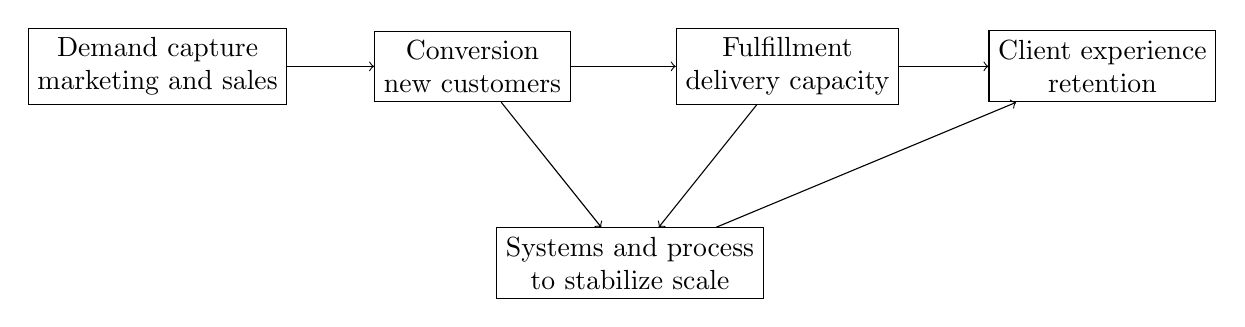
\begin{tikzpicture}
\node[draw, rectangle, align=center] (m) at (0,0) {Demand capture\\marketing and sales};
\node[draw, rectangle, align=center] (c) at (4,0) {Conversion\\new customers};
\node[draw, rectangle, align=center] (f) at (8,0) {Fulfillment\\delivery capacity};
\node[draw, rectangle, align=center] (x) at (12,0) {Client experience\\retention};
\node[draw, rectangle, align=center] (p) at (6,-2.5) {Systems and process\\to stabilize scale};
\draw[->] (m) -- (c);
\draw[->] (c) -- (f);
\draw[->] (f) -- (x);
\draw[->] (c) -- (p);
\draw[->] (f) -- (p);
\draw[->] (p) -- (x);
\end{tikzpicture}
\caption{Transcript-derived scaling chain. Growth begins with captured demand, but it survives only if fulfillment and process keep the client experience from breaking.}
\end{figure}

The chapter can afford a little abstraction here because the lecture itself is already abstracting. Let $M$ denote demand capture, let $F$ denote fulfillment capacity, and let $X$ denote the quality of the client experience. The spoken point is that $M$ can rise faster than $F$, in which case $X$ falls. The business looks successful from the top of the funnel and unstable from the inside. That is why the speaker immediately adds a second requirement: someone with operational experience must come in and build systems and process.

From here the lecture widens outward from operating mechanics to the economics of self-investment. The entrepreneur says the best advice he received was to bet on himself. He recalls earning only $19{,}000$ a year while already thinking of himself as rich in a forward-looking sense. This is not empty affirmation in the context of the lecture. It is a claim about state variables. Present income is not the thing being optimized; capacity, skill, and self-reinvestment are. The logic is delayed rather than immediate.

A short break follows in which the video promotes the School of Mentors community. Structurally this is only an intermission. When the lecture resumes, it does so without abandoning the prior line of thought. We are still asking how scale is built, only now through a different business form.

\section{Implementation, Debt, and Sales Structure}

The industrial distributor provides the next major refinement. The origin story is older and slower: forty years of entrepreneurship, apprenticeship inside the father's business, an early company in electronics, and eventually a distributorship whose good years reach roughly $250\,\mathrm{M}$ in revenue. The tone changes here. We are no longer in the fast-growth world of a three-year-old company. We are in the longer arc of implementation, hiring, financing, and channel structure.

\subsection{Question \& Answer}

\paragraph{Question.} What matters more: product or distribution?

\paragraph{Answer.} The lecture deliberately sets up this binary only to reject it. The interviewee says neither, taken alone, is decisive. Products may be fine. Distribution may exist. Yet the business can still fail. The controlling variable is implementation. This is an important move. It prevents us from mistaking a category label for a mechanism.

The interview then pushes this insight outward. How does one scale from eight figures to nine? Get the right people on the bus. Then business plan, financing, and partners. How does debt enter? Yes, banks matter, but banks do not lend easily to small businesses without prior money or insider status. The lecture's picture of financing is not utopian. It is adversarial. Private equity and strategic rollups have already occupied many industries, and the bank's door is not equally open to outsiders.

At this point the lecture introduces one of its sharpest definitions.

\begin{definition}
A hunter generates new business. A farmer grows business inside existing accounts. The lecture's claim is that a mature sales organization needs both.
\end{definition}

The clean schematic identity is
\begin{equation}
S_{\text{total}} = S_{\text{hunter}} + S_{\text{farmer}}.
\end{equation}
This is not an accounting formula from the firm. It is a note-taking device that preserves the speaker's distinction. One part of the sales function searches outward; the other deepens what has already been won. The business cannot be understood if we collapse those roles into a single vague notion of selling.

The interview closes with a broader cultural complaint: the older ethic is summarized as ``I earn,'' while the newer pathology is summarized as ``I deserve.'' Whether or not we agree with the diagnosis in full, its function inside the lecture is clear. It converts the long industrial case into a moral reading of labor, entitlement, and discipline. We begin with implementation inside the firm and end with implementation inside the person.

\section{Cash Flow, Contracts, and Leadership Under Pressure}

After a noisy transition, the lecture lands on the final major case: an ex-military operator who says he was broke in the military, then began buying and selling businesses, moved overseas, and later worked across private equity, venture capital, and investment banking. Here the lecture stops circling the central constraint and names it directly.

\subsection{Question \& Answer}

\paragraph{Question.} What is the most common mistake that keeps businesses from surviving?

\paragraph{Answer.} Cash flow. The answer comes instantly, and the lecture repeats it for emphasis. Revenue is useful, but cash is the quantity that decides whether the doors remain open.

The natural update rule is the plain bookkeeping identity
\begin{equation}
C_{t+1} = C_t + I_t - O_t,
\end{equation}
with $C_t$ the cash balance at time $t$, $I_t$ inflows, and $O_t$ outflows. The speaker then adds the horizon: build an eighteen-month model. In our notation,
\begin{equation}
H = 18\,\mathrm{months}.
\end{equation}
What matters is not merely that a business reports annual revenue $R$, but that cash remain positive across the planning window:
\begin{equation}
C_t > 0 \qquad \text{for all } t \in [0,H].
\end{equation}

We may spell out the implication in the simplest possible way. If at some month the obligations exceed opening cash plus incoming cash,
\begin{equation}
O_t > C_t + I_t,
\end{equation}
then
\begin{equation}
C_{t+1} < 0.
\end{equation}
That is the lecture's hard edge. A firm can sound healthy in the language of revenue and still fail at the level of liquidity.

A short worked derivation is enough for the notes:
\begin{enumerate}
\item Put the business on a monthly grid $t=0,1,\dots,H$.
\item Update cash by $C_{t+1}=C_t+I_t-O_t$.
\item Demand that $C_t>0$ throughout the horizon.
\item Conclude that survival is a path condition on cash, not a single annual revenue number.
\end{enumerate}

From here the lecture broadens again. Scale requires focus, even at the expense of balance. Financial advice becomes contractual advice: nothing is real until there is a contract, keep everything above the table, do nothing illegal, immoral, or unethical. Negotiation advice becomes restraint: do not talk past the sale. Sales advice becomes role clarity: he is not the sales guy; his strength is leadership and motivation. Military background becomes transferable structure: discipline, gratitude, meditation, and the ability to absorb loss without collapsing.

The closing remarks then return to a refrain we already heard in the opening montage. At sixty, the operative words are still focus and discipline. If one could speak backward to the younger self, the message is not a new tactic but an endurance principle: stay in the fight.

\section{Summary}

This lecture gives us a sequence of business invariants rather than a single doctrine. First, wealth is repeatedly traced back to ownership structure. Second, scale is shown to be a two-stage problem: demand capture first, fulfillment and process immediately after. Third, the false binaries -- product versus distribution, revenue versus survival, sales versus leadership -- are dissolved by more careful distinctions. Fourth, cash flow emerges as the final gatekeeper. If cash goes negative, the story ends, no matter how attractive the revenue line may look.

The lecture closes, as it began, with compression. Focus, discipline, communication, implementation, retained ownership when possible, operational systems, contract clarity, negotiation restraint, gratitude, and persistence: these are not separate slogans. They are the recurrent control parameters of the episode. The chapter should therefore preserve the field-report rhythm of the lecture while making those parameters explicit enough to think with.